\documentclass[../final_report.tex]{subfiles}
\usepackage{subfiles}
\graphicspath{{../../Lab3/plots/}}
\begin{document}


Σε αυτή την άσκηση, επιστρέφουμε πίσω στην ανάλυση της παραλληλοποίησης του αλγορίθμου K-means. Στην naive 
έκδοση, υπάρχει το ζήτημα της ανανέωσης των μεταβλητών newClusters και newClustersSize, οι οποίες δείχνουν
τις μεταβολές των κέντρων των Cluster και το μέγεθος αυτών. Εφόσον λειτουργούμε με διαμοιραζόμενα δεδομένα,
η ανανέωση αυτών των μεταβλητών πρέπει να γίνει ατομικά, δηλαδή από κάθε νήμα ξεχωριστά.

Το κομμάτι κώδικα στο οποίο γίνεται αυτή η ανανέωση είναι το critical section του προβλήματος.

\subsubsection*{K-Means Naive - Critical Section}
\begin{lstlisting}
    // update new cluster centers : sum of objects located within 
    lock_acquire(lock);
    newClusterSize[index]++;
    for (j=0; j<numCoords; j++){
        newClusters[index*numCoords + j] += objects[i*numCoords + j];
    }
    lock_release(lock);
\end{lstlisting}

Η δημιουργία αυτού του χώρου mutual exclusion μπορεί να γίνει είτε με χρήση locks ή με χρήση
των pragma του OpenMP \textbf{\#pragma omp atomic/critical}

\subsection{Mutual Exclusion με χρήση κλειδαριών}

Στην ανάλυση που θα κάνουμε, πρέπει να πάρουμε υπόψιν τα NUMA χαρακτηριστικά της 
αρχιτεκτονικής που χρησιμοποιούμε. Όλα τα κλειδώματα που θα αναλύσουμε έχουν μειονέκτημα
ότι μοιράζονται το entity του lock. Η ανανέωση της τιμής του lock θα προκαλέσει cache invalidation
και θα εφαρμοστεί το MESI πρωτόκολλο για να υπάρξει συνάφεια μνήμης. Εφόσον έχουμε και NUMA χαρακτηριστικά
αλλά και cache coherence, την αρχιτεκτονική αυτή την αποκαλόυμε cc-NUMA.


Τα locks που θα εξετάσουμε είναι τα εξής:

\begin{description}
    \item [Pthread - Mutex]
    \item [Pthread - Spinlock]
    \item [Test-and-Set (TAS)]
    \item [Test-Test-and-Set (TTAS)]
    \item [Array Based Lock] 
    \item [CLH Lock] 
\end{description}

Παρουσιάζουμε και την εκδοχή χωρίς κλειδώματα για λόγους σύγκρισης.

\subsubsection{Εκτέλεση χωρίς κλείδωμα}

Η εκτέλεση χωρίς κλειδώματα θα προσφέρει λάθος αποτελέσματα καθώς κανείς δεν μας
καθιστά σίγουρο ότι δεν μπορούν 2 νήματα ή παραπάνω να επεξεργαστούν την ίδια μεταβλητή και 
κάποιο να "ακυρώσει" την δράση ενός άλλου νήματος.

\begin{figure}[H]
    \centering
        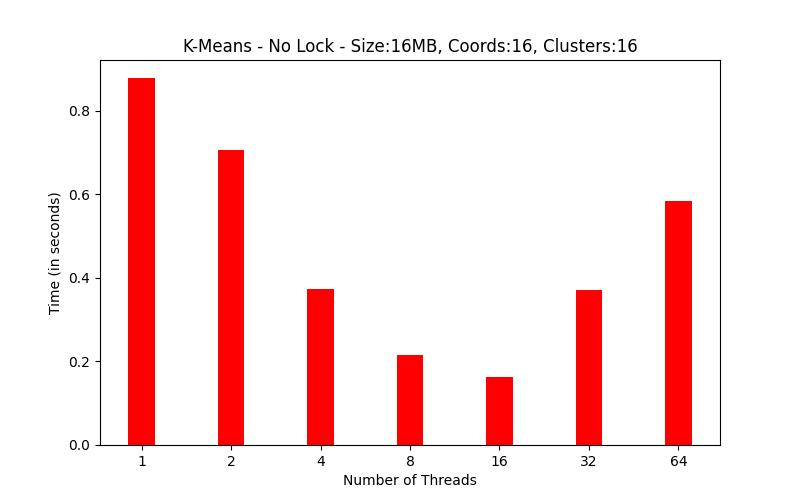
\includegraphics[scale=0.4]{outFilesAffinityMouliko/plots/kmeans_locks_nosync.jpg}
        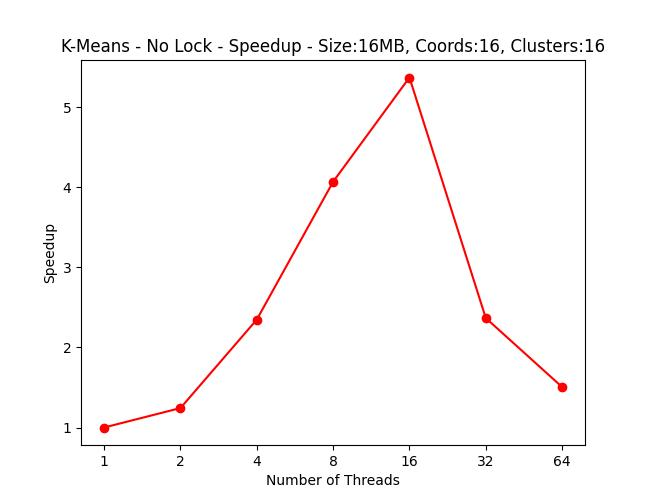
\includegraphics[scale=0.4]{outFilesAffinityMouliko/plots/kmeans_locks_nosync_speedup.jpg}
    \caption{K-Means Naive - No Sync}
    \label{fig:K-Means Naive - No Sync}
\end{figure}

Περιμένουμε ο βέλτιστος χρόνος εκτέλεσης να είναι από αυτή την εκδοχή αφού δεν υπάρχει το overhead
του locking.

\subsubsection*{Best Time - No Sync}
0.1635s - 16 Threads

\subsubsection{PThread - Mutex}

Το mutex είναι από τις πιο απλές μορφές mutual exclusion lock. Το συγκεκριμένο lock έχει μόνο 2 καταστάσεις,
locked και unlocked. Μόνο ένα νήμα επιτρέπεται να κατέχει το lock κάθε στιγμή. Αν ένα νήμα προσπαθήσει να 
αποκτήσει ένα ήδη κλειδωμένο lock, το νήμα θα γίνει blocked μέχρι να απελευθερωθεί το lock.

Όταν απελευθερωθεί, ένα από τα νήματα που περιμένουν θα επιλεχθεί να μπει στο κρίσιμο τμήμα του
προγράμματος.

\begin{figure}[H]
    \centering
        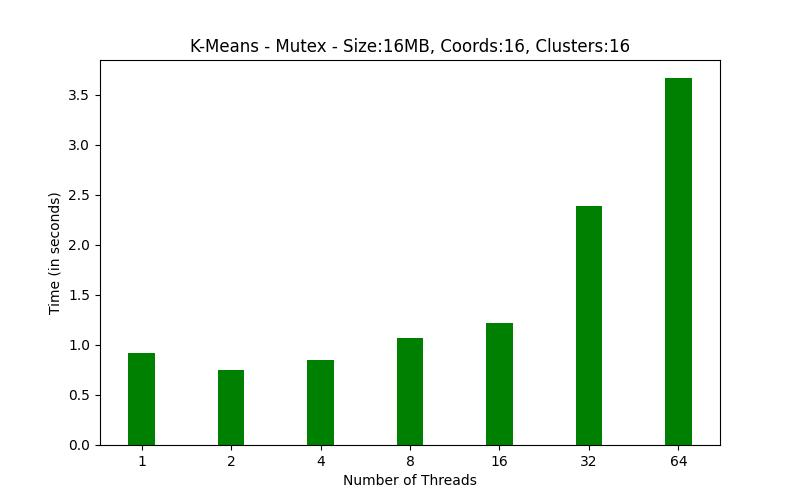
\includegraphics[scale=0.4]{outFiles/plots/kmeans_locks_pthread_mutex.jpg}
        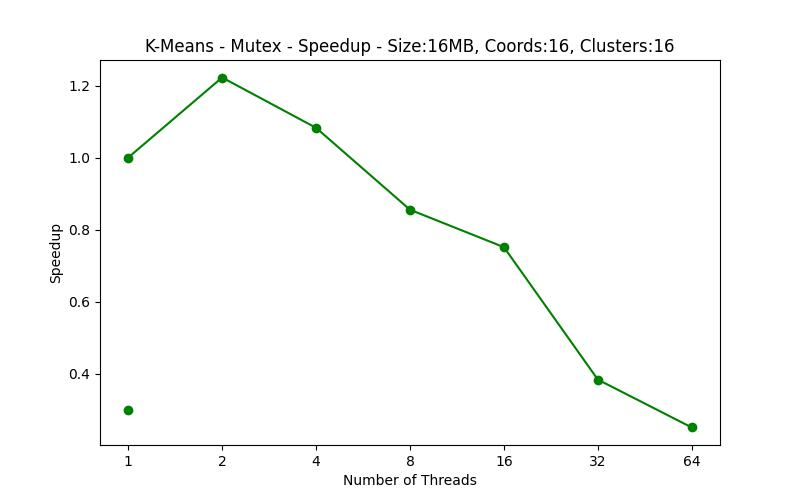
\includegraphics[scale=0.4]{outFiles/plots/kmeans_locks_pthread_mutex_speedup.jpg}
    \caption{K-Means Naive - PThread - Mutex}
    \label{fig:K-Means Naive - PThread - Mutex}
\end{figure}

Φαίνεται ότι ο χρόνος εκτέλεσης επηρεάζεται πολύ από την χρήση του κλειδώματος. Το overhead
που προσθέτει το συνεχόμενο κλείδωμα/ξεκλείδωμα μαζί με τα συνεχόμενα MESI invalidations
καθιστούν το mutex lock μια κακή επιλογή όταν έχουμε σύστημα με πολλούς πυρήνες, πολλά MESI nodes και συχνά
κλειδώματα.

Άλλος συντελεστής που επηρεάζει την απόδοση των mutex είναι ότι απαιτείται context switch για τις
λειτουργίες του. Η χρησιμότητα τους φαίνεται σε άλλα προγράμματα με μεγαλύτερα critical sections.
Επίσης, είναι επιτρεπτό ένα νήμα να πέσει για ύπνο όσο περιμένει το lock, δεν θα προκαλέσει deadlock.

\subsubsection*{Best Time - PThread - Mutex}
0.7506s - 2 Threads

\subsubsection{PThread - Spinlock}

Τα spinlock διαφέρουν αρκετά από τα mutexes. Αντί να γίνει blocked το νήμα που προσπαθεί να πάρει το ήδη
κλειδωμένο lock, θα μπεί σε busy-wait loop μέχρι να απελευθερωθεί το lock. Αυτό σημαίνει ότι δεν γίνεται
context switch στην λειτουργία τους. Η υλοποίηση της βιβλιοθήκης pthread χρησιμοποιεί είτε εντολή
atomic\_exchange (αν υποστηρίζεται από το υλικό) ή μια weak εντολή compare-and-swap (αν δεν υποστηρίζεται το atomic\_exchange).

\begin{figure}[H]
    \centering
        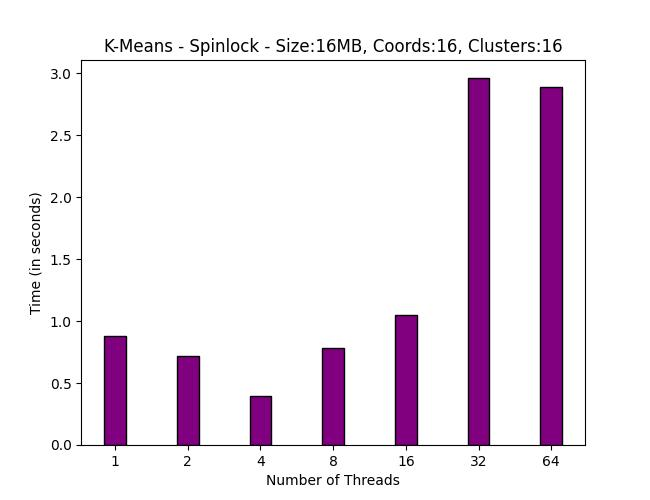
\includegraphics[scale=0.4]{outFilesAffinityMouliko/plots/kmeans_locks_pthread_spin.jpg}
        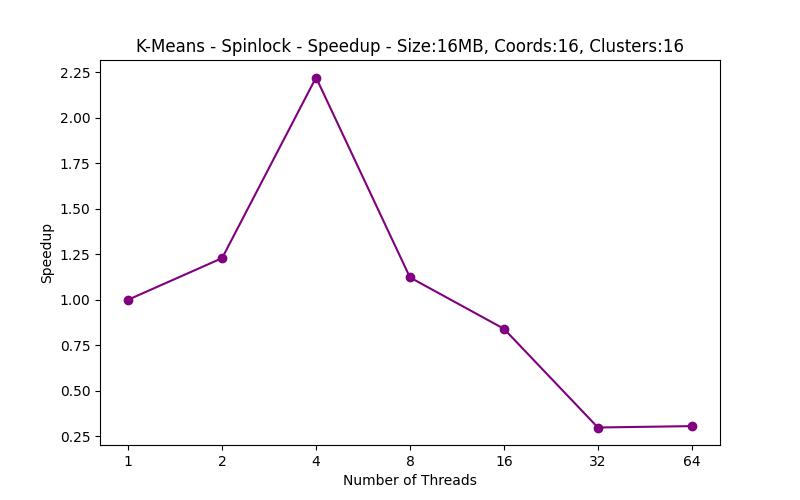
\includegraphics[scale=0.4]{outFilesAffinityMouliko/plots/kmeans_locks_pthread_spin_speedup.jpg}
    \caption{K-Means Naive - PThread - Spinlock}
    \label{fig:K-Means Naive - PThread - Spinlock}
\end{figure}

Παρατηρούμε πολύ καλύτερη απόδοση συγκριτικά με το κλείδωμα με mutex. Η απουσία του context switching για το κλείδωμα και ξεκλείδωμα και 
το γεγονός ότι το κρίσιμο μονοπάτι του συγκεκριμένου προβλήματος είναι μικρό ευνοεί σημαντικά τα spinlock.

Για απλά κλειδώματα στα οποία τα νήματα δεν χρειάζεται να περιμένουν πολύ ώρα για να λάβουν το lock, τα spinlock
είναι μια καλή επιλογή.

\subsubsection*{Best Time - PThread - Spinlock}
0.3960s - 4 Threads


\subsubsection{Test-and-Set (TAS)}

Τα κλειδώματα Test-and-Set ακολουθούν την εξής λογική:

- Έστω η μέθοδος "Test", η οποία ελέγχει αν το lock έχει παρθεί από κάποιο thread. Αν η κλειδαριά
είναι ελέυθερη, η "Test" επιστρέφει False. Αν όχι, επιστρέφει True.

- Το νήμα που καλεί την "Test", όχι μόνο διαβάζει την τιμή του lock, αλλά αννανεώνει κιόλας το lock 
με την τιμή που μόλις διάβασε

\begin{figure}[H]
    \centering
        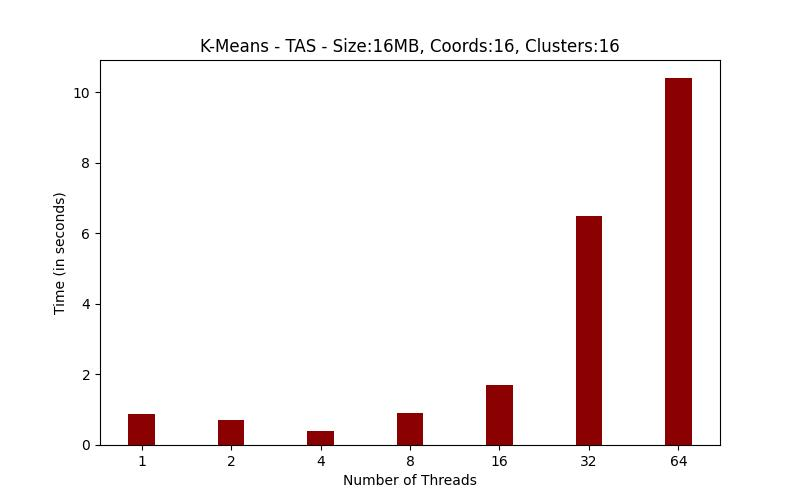
\includegraphics[scale=0.4]{outFilesAffinityMouliko/plots/kmeans_locks_tas.jpg}
        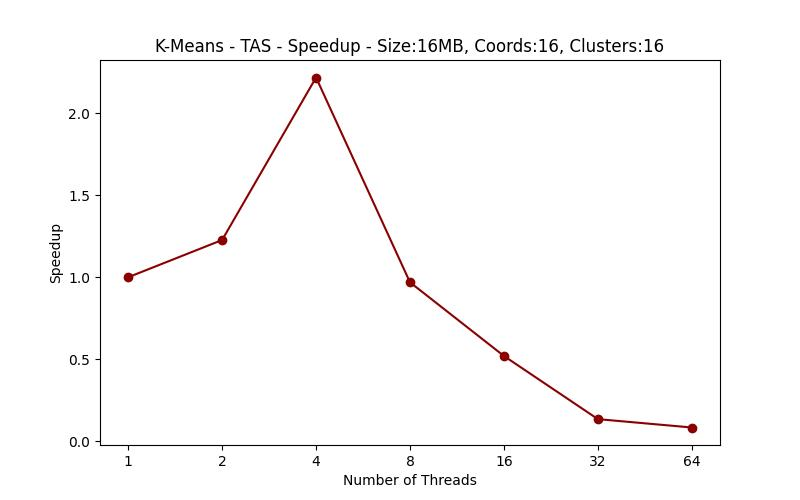
\includegraphics[scale=0.4]{outFilesAffinityMouliko/plots/kmeans_locks_tas_speedup.jpg}
    \caption{K-Means Naive - TAS}
    \label{fig:K-Means Naive - TAS}
\end{figure}


Για μικρό αριθμό νημάτων, παρατηρούμε ότι τα κλειδώματα TAS έχουν επιτρεπτή απόδοση.
Το overhead τους είναι πολύ μικρό καθώς απλώς εκτελούν έναν ατομικό έλεγχο και ανανέωση
μεταβλητής.

Η κατάσταση αυτή αλλάζει σημαντικά όταν αυξάνουμε τον αριθμό νημάτων. Εδώ, αναφερόμαστε πάλι
στα NUMA χαρακτηριστικά των επεξεργαστών που χρησιμοποιούμε, καθώς και στην ανάγκη για cache
coherence. Με τα TAS κλειδώματα, εκτελόυμε περιττά
cache invalidations ανανεώνοντας συνεχώς την τιμή του lock καθώς κάνουμε τον έλεγχο. Έχουμε 
υπερβολική "κίνηση" στον δίαυλο μνήμης των επεξεργαστών. Επίσης, ειδικά στην περίπτωση που 
χρησιμοποιούμε 64 νήματα, υπάρχουν και οι ακραίες περιπτώσεις που πρέπει 2 νήματα που απέχουν
την μεγαλύτερη δυνατή απόσταση μεταξύ τους να χρειαστέι να κάνουν Modify (και άρα να γίνουν Invalidated
τα υπόλοιπα). Αυτή η μεταφορά δεδομένων από τα πιο μακρινά NUMA nodes καταστρέφει την απόδοση.

Τα κλειδώματα TAS έχουν την χειρότερη απόδοση από όλα τα κλειδώματα. Το "σφάλμα" τους είναι 
ξεκάθαρο και επιλύνεται από το επόμενο κλείδωμα.

\subsubsection*{Best Time - Test-and-Set}
0.3960s - 4 Threads


\subsubsection{Test-Test-and-Set (TTAS)}

Σε αντίθεση με το TAS κλείδωμα, το TTAS κλείδωμα \textbf{ΔΕΝ} αλλάζει την τιμή του lock αν το βρει
κλειδωμένο, αλλά το αφήνει \textbf{LOCKED}. Γίνεται συνεχόμενα έλεγχος για αν το lock είναι ελεύθερο
από κάποιο νήμα αλλά αυτό δεν σημαίνει ότι με το που αλλάξει η τιμή σε \textbf{UNLOCKED} το νήμα
αυτό θα πάρει το lock. Για αυτό, χρειάζεται να τρέξουμε άλλη μια φορά την μέθοδο getAndSet(true) (δηλαδή την
"μέθοδο" "Test") για να πάρει το lock. Αν αποτύχει η συγκεκριμένη μέθοδος και βρει πάλι κλειδωμένο το lock, σημαίνει ότι
κάποιο άλλο νήμα πρόλαβε να παραλάβει την κλειδαριά, και το νήμα που προσπάθησε ξανά τρέχει συνεχόμενους 
ελέγχους.


\begin{figure}[H]
    \centering
        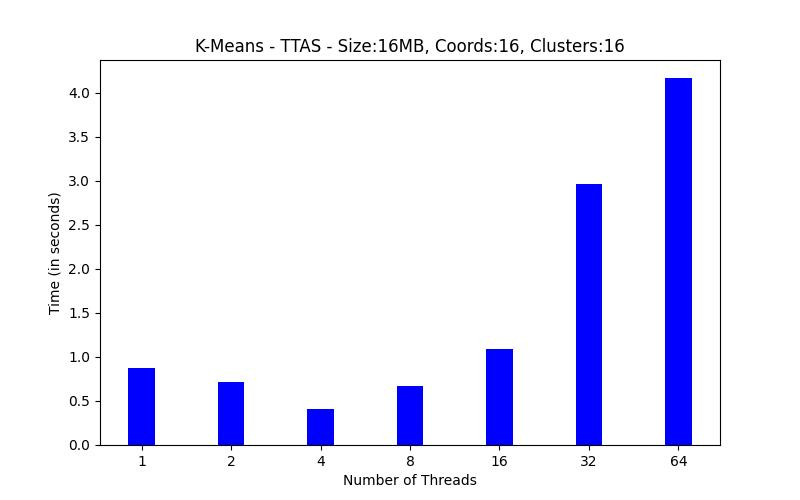
\includegraphics[scale=0.4]{outFilesAffinityMouliko/plots/kmeans_locks_ttas.jpg}
        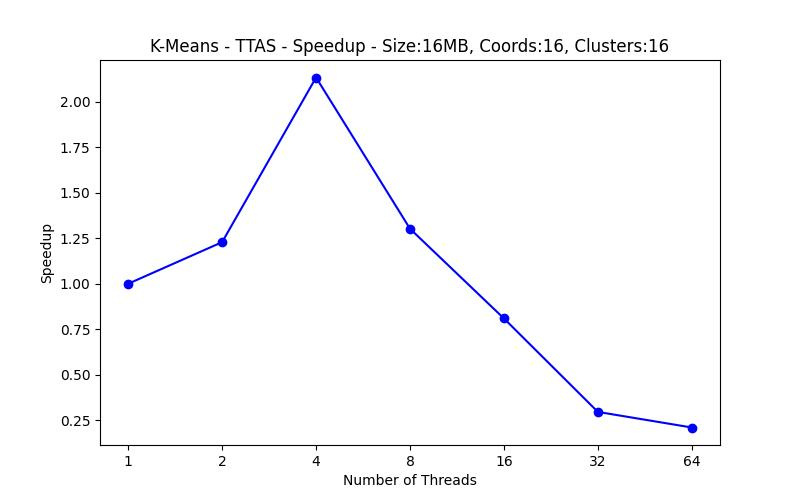
\includegraphics[scale=0.4]{outFilesAffinityMouliko/plots/kmeans_locks_ttas_speedup.jpg}
    \caption{K-Means Naive - TTAS}
    \label{fig:K-Means Naive - TTAS}
\end{figure}

Το overhead των TTAS κλειδωμάτων είναι ελάχιστα μεγαλύτερο από τα TAS κλειδώματα και άρα σε 
μικρό αριθμό νημάτων, τα TTAS είναι ελάχιστα χειρότερα από τα TAS.

Χρησιμοποιώντας περισσότερα νήματα, παρατηρούμε ότι η απόδοση είναι 2 φορές καλύτερη από τα 
TAS κλειδώματα. Ακόμα όμως και με αυτή την αλλαγή, η επίδοση των TTAS κλειδωμάτων, δεν είναι και η
καλύτερη. 

Όταν πολλά νήματα "παλέυουν" για την απόκτηση μιας κλειδαριάς, λέμε ότι υπάρχει μεγάλος ανταγωνισμός.
Αν συχνά ένα νήμα αποτυγχάνει να αποκτήσει το lock έχοντας όμως ήδη περάσει το πρώτο "Test" στάδιο,
πρέπει για λίγο χρόνο να σταματήσει να προσπαθεί να αποκτησει το lock γιατί έτσι μειώνεται η 
κινητικότητα στην δίαυλο μνήμης. Την λογική αυτή ακολουθούν τα επόμενα κλειδώματα.

\subsubsection*{Best Time - Test-Test-and-Set}
0.4121s - 4 Threads

\subsubsection{Array Based Lock}

Το συγκεκριμένο κλείδωμα υλοποιείται ως ένα queue. Τα νήματα μοιράζονται μια μεταβλητή, την ουρά,
η οποία δείχνει ποιος κατέχει την κλειδαριά. Για να αποκτήσει ένα νήμα το lock, αυξάνει κατά 1 την 
μεταβλητή της ουράς. Το μέγεθος αυτό δείχνει το ποιο νήμα έχει τον έλεγχο. Χρησιμοποιώντας αυτόν τον
αριθμό ως index, μια boolean τιμή δείχνει αν ένα lock είναι ελεύθερο ή δεσμευμένο. Αν είναι true, τότε επιτρέπεται
το νήμα να πάρει το lock.

Τα νήματα κάνουν spin μέχρι το slot τους να γίνει true. Για να απελευθερωθεί το lock, το κάθε νήμα
καθιστά την δική τους θέση ως false και κάνουν set την επόμενη θέση σε true.

\begin{figure}[H]
    \centering
        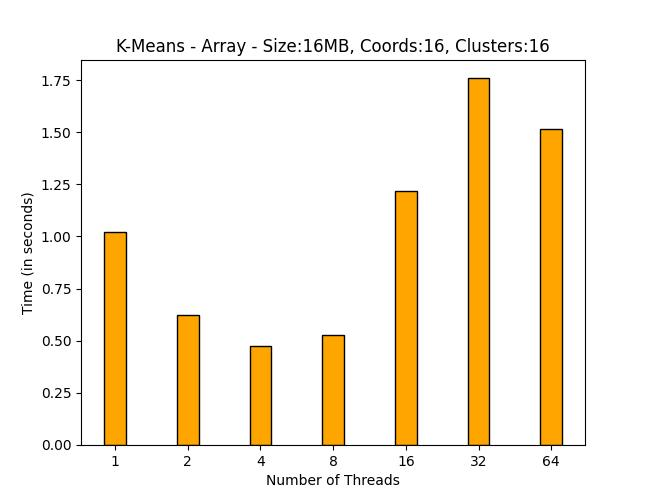
\includegraphics[scale=0.4]{outFilesCores/plots/kmeans_locks_array.jpg}
        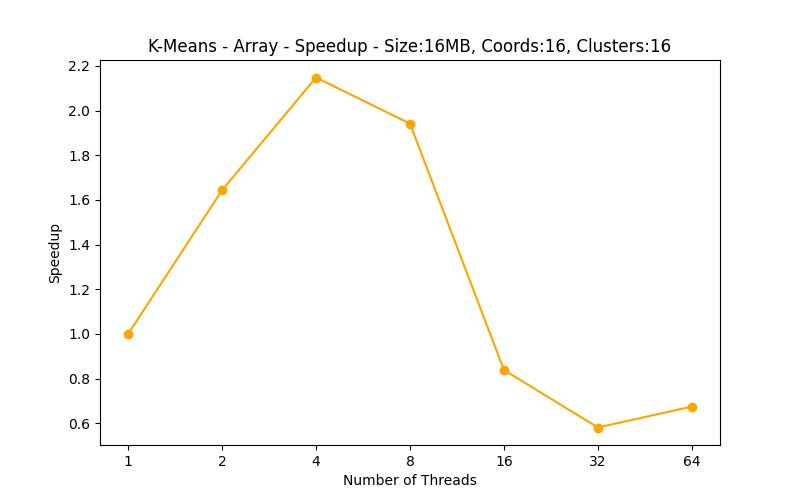
\includegraphics[scale=0.4]{outFilesCores/plots/kmeans_locks_array_speedup.jpg}
    \caption{K-Means Naive - Array Based Lock}
    \label{fig:K-Means Naive - Array Based Lock}
\end{figure}

Ο συγκεκριμένος τύπος κλειδώματος είναι ο πρώτος που επιχειρεί να είναι NUMA/cache coherent aware. Η τιμή που δείχνει
την θέση του κάθε νήματος (mySlotIndex) είναι τοπική για κάθε νήμα. Δηλαδή, τα νήματα κάνουν spin σε μια θέση 
μνήμης που είναι τοπική. Έτσι, δεν προκαλείται coherence traffic χωρίς λόγο. Αν και ο boolean πίνακας είναι 
διαμοιραζόμενος, τα νήματα δεν "παλεύουν" να αποκτήσουν πρόσβαση σε αυτή την θέση μνήμης καθώς κάνουν
spin στις τοπικές θέσεις τους, μειώνοντας έτσι και το invalidation traffic.

Το array lock έχει το μειονέκτημα ότι πρέπει να προσέχουμε για φαινόμενα false sharing. Εφόσον ο boolean πίνακας που 
δείχνει την κατάσταση του lock είναι διαμοιραζόμενος, θα υπάρχει σχεδόν σίγουρα false sharing. False sharing 
σημαίνει ότι 2 ή περισσότερα νήματα μοιράζονται ίδια cache lines αλλά επεξεργάζονται διαφορετικές μεταβλητές.
Η ευκολότερη λύση είναι να χρησιμοποιήσουμε padding.

Άλλο ένα πλεονέκτημα είναι ότι είναι πολύ δίκαιο lock και δεν παρατηρείται starvation. Λόγω της σχεδίασης του lock ώς
ουρά, εκτελείται first-come-first-served σειρά εκτέλεσης.

Παρατηρούμε πολύ καλύτερους χρόνους για αριθμό νημάτων πάνω από 8, τουλάχιστον συγκριτικά με τις προηγούμενες υλοποιήσεις. 
Πάλι όμως, το πρόβλημα δεν κλιμακώνει για πάνω από 8 νήματα. 

\subsubsection*{Best Time - Array Based Lock}
0.4755s - 4 Threads

\subsubsection{CLH Lock}

Η τελευταία βελτίωση που θα μελετήσουμε είναι για να μειωθεί η ανάγκη για μνήμη που απαιτεί το array lock.

Το CLH lock ακολουθεί την λογική του array lock, δηλαδή ότι τα νήματα κάνουν spin τοπικά. Αντί για ουρά,
χρησιμοποιεί μια σχεδίαση linked list. Το κάθε νήμα έχει τοπικά ένα QNode που δείχνει την κατάσταση του.
Αν η boolean τιμή locked είναι true, τότε το νήμα είτε έχει έλεγχο του lock ή περιμένει για αυτόν. Αν είναι false,
έχει αφήσει το lock. Κάθε νήμα αναφέρεται στο node του προηγούμενου νήματος με μία τοπική μεταβλητή.

Για να γίνει locked ή unlocked η κλειδαριά, χρησιμοποιείτε παρόμοια λογική με το array lock, απλά αυτή την φορά
αντί να κάνουμε increment την θέση του πίνακα που κοιτάζει την κατάσταση του νήματος, το κάθε νήμα
γίνεται locked από μόνο του και μετά θέτει το node του ως το tail του queue. Για να απελευθερωθεί το lock, 
θέτει τον εαυτό του ως unlocked και χρησιμοποιεί το node του προηγούμενου νήματος ως το νέο node του για 
τα επόμενα κλειδώματα.

\begin{figure}[H]
    \centering
        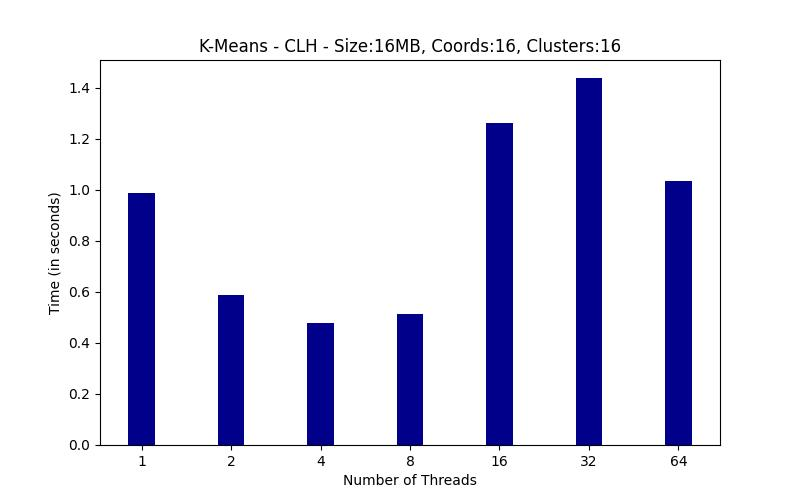
\includegraphics[scale=0.4]{outFilesCores/plots/kmeans_locks_clh.jpg}
        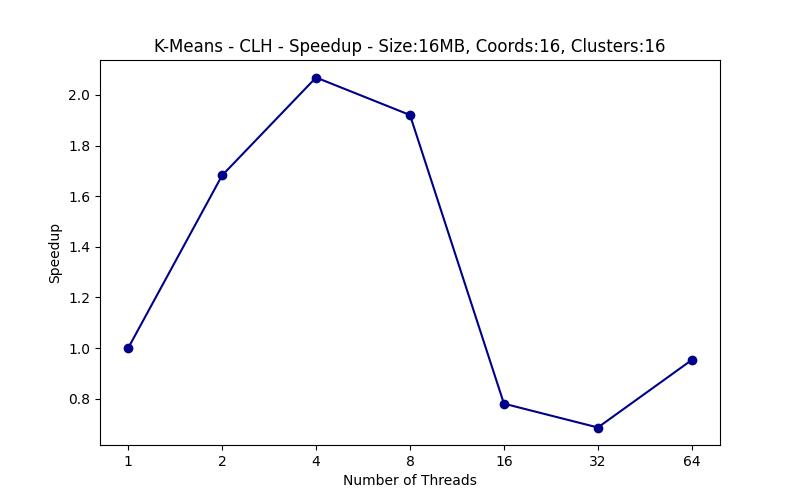
\includegraphics[scale=0.4]{outFilesCores/plots/kmeans_locks_clh_speedup.jpg}
    \caption{K-Means Naive - CLH Lock}
    \label{fig:K-Means Naive - CLH Lock}
\end{figure}

Η προγραμματιστική δυσκολία του CLH Lock είναι ξεκάθαρη, με εμφανή αποτελέσματα όμως. Έχει την πιο
ισορροπημένη απόδοση συγκριτικά με όλες τις υλοποιήσεις. Ακόμα και σε μεγάλο αριθμό νημάτων, δεν μειώνεται η 
απόδοση του σε μεγάλο βαθμό. Πάλι όμως, δεν παρατηρείται κλιμάκωση για πάνω από 8 νήματα. 

\subsubsection*{Best Time - CLH Lock}
0.4768s - 4 Threads

\subsubsection*{All Times}

\begin{figure}[H]
    \centering
        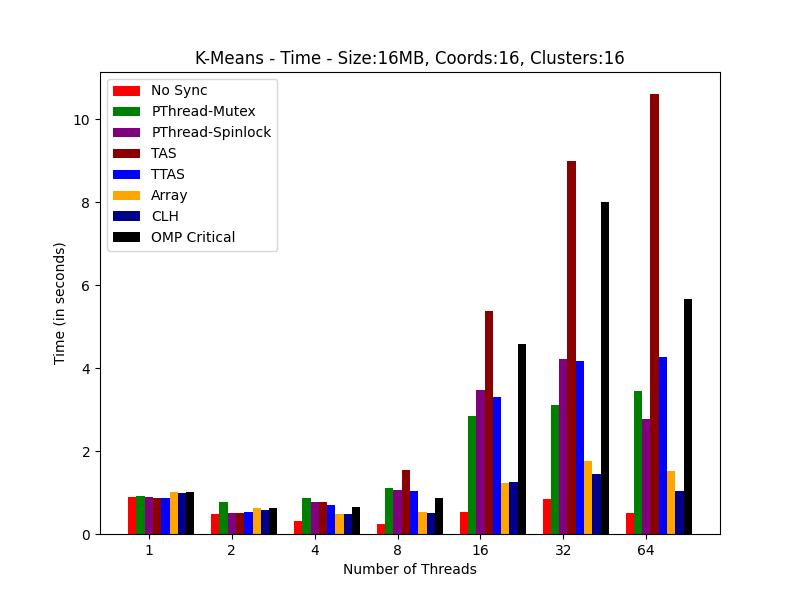
\includegraphics[scale=0.4]{outFilesCores/plots/kmeans_locks_all.jpg}
        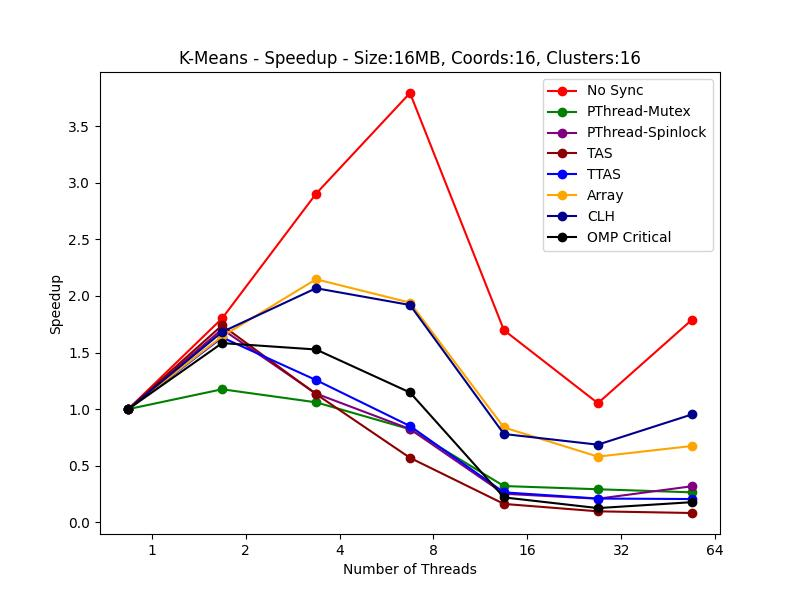
\includegraphics[scale=0.4]{outFilesCores/plots/kmeans_locks_all_speedup.jpg}
    \caption{K-Means Naive - All Locks}
    \label{fig:K-Means Naive - All Locks}
\end{figure}


\subsection{Mutual Exclusion με χρήση critical/atomic pragma}

Είχα πάει σε πρόγραμμα Erasmus+ και δεν πρόλαβα να κάνω αυτό το ερώτημα καθώς είχε πέσει ο sandman την ώρα που το έστελνα.
Θα το παραδώσω μαζί με το επόμενο ερώτημα, χίλια συγγνώμη.

\end{document}